\documentclass[12pt]{article}
%--------------------   start of the 'preamble'
%
\usepackage{graphicx,amssymb,amstext,amsmath,color}
\usepackage{grffile}
\usepackage[margin=2cm]{geometry}
\usepackage{abstract}
\usepackage{setspace}
\usepackage[footnotesize,bf]{caption}

% TABLE
\usepackage{multicol,hhline,colortbl,multirow}
\usepackage{braket}
\usepackage{siunitx}
\usepackage{hyperref}
\usepackage{authblk}
\usepackage{siunitx}
\usepackage{adjustbox}
\usepackage{mathrsfs}
%%\usepackage[sort&compress]{natbib}
%%\bibpunct{(}{)}{,}{a}{, }{;}
%
\usepackage[sort&compress]{natbib}
\bibpunct{[}{]}{,}{s}{}{;}


\definecolor{gray}{gray}{0.8}
\def\mobunits{\square\centi\meter\per\volt\per\second}
\def\gcm{\gram\per\cubic\centi\meter}
\def\ccg{\cellcolor{gray}}

\renewcommand{\labelitemii}{$\circ$}
\renewcommand{\bibname}{References}


\title{What Effect Does Fully Equilibrating After Fine-Graining Have on the Charge Transport Properties?}
\author{Matthew Jones}
\date{\today}

\begin{document}
\maketitle

\section{Simulations}

The previous lot of runs were not properly equilibrated, even though the potential energies looked good.
The temperature was found to oscillate wildly, and the strong dependence on the value of the thermostat coupling $\tau$ made conclusions difficult to extract.
Simulations run over Thanksgiving had velocities initialized based on the temperature of the system, to make things easier on the thermostat.
The entire fine-graining process now takes 48 hours.
The results are presented below.


\section{Equilibration}


\textcolor{red}{The T2.5 system did not run correctly, and will need to be rerun. That datapoint is therefore missing.}


\textcolor{red}{Even with the initialized velocities, I still get the weird oscillations in PE and Temperature. Is this some effect of having small timesteps (1E-5 for the final phase)?}


\begin{figure}[h!]\centering
	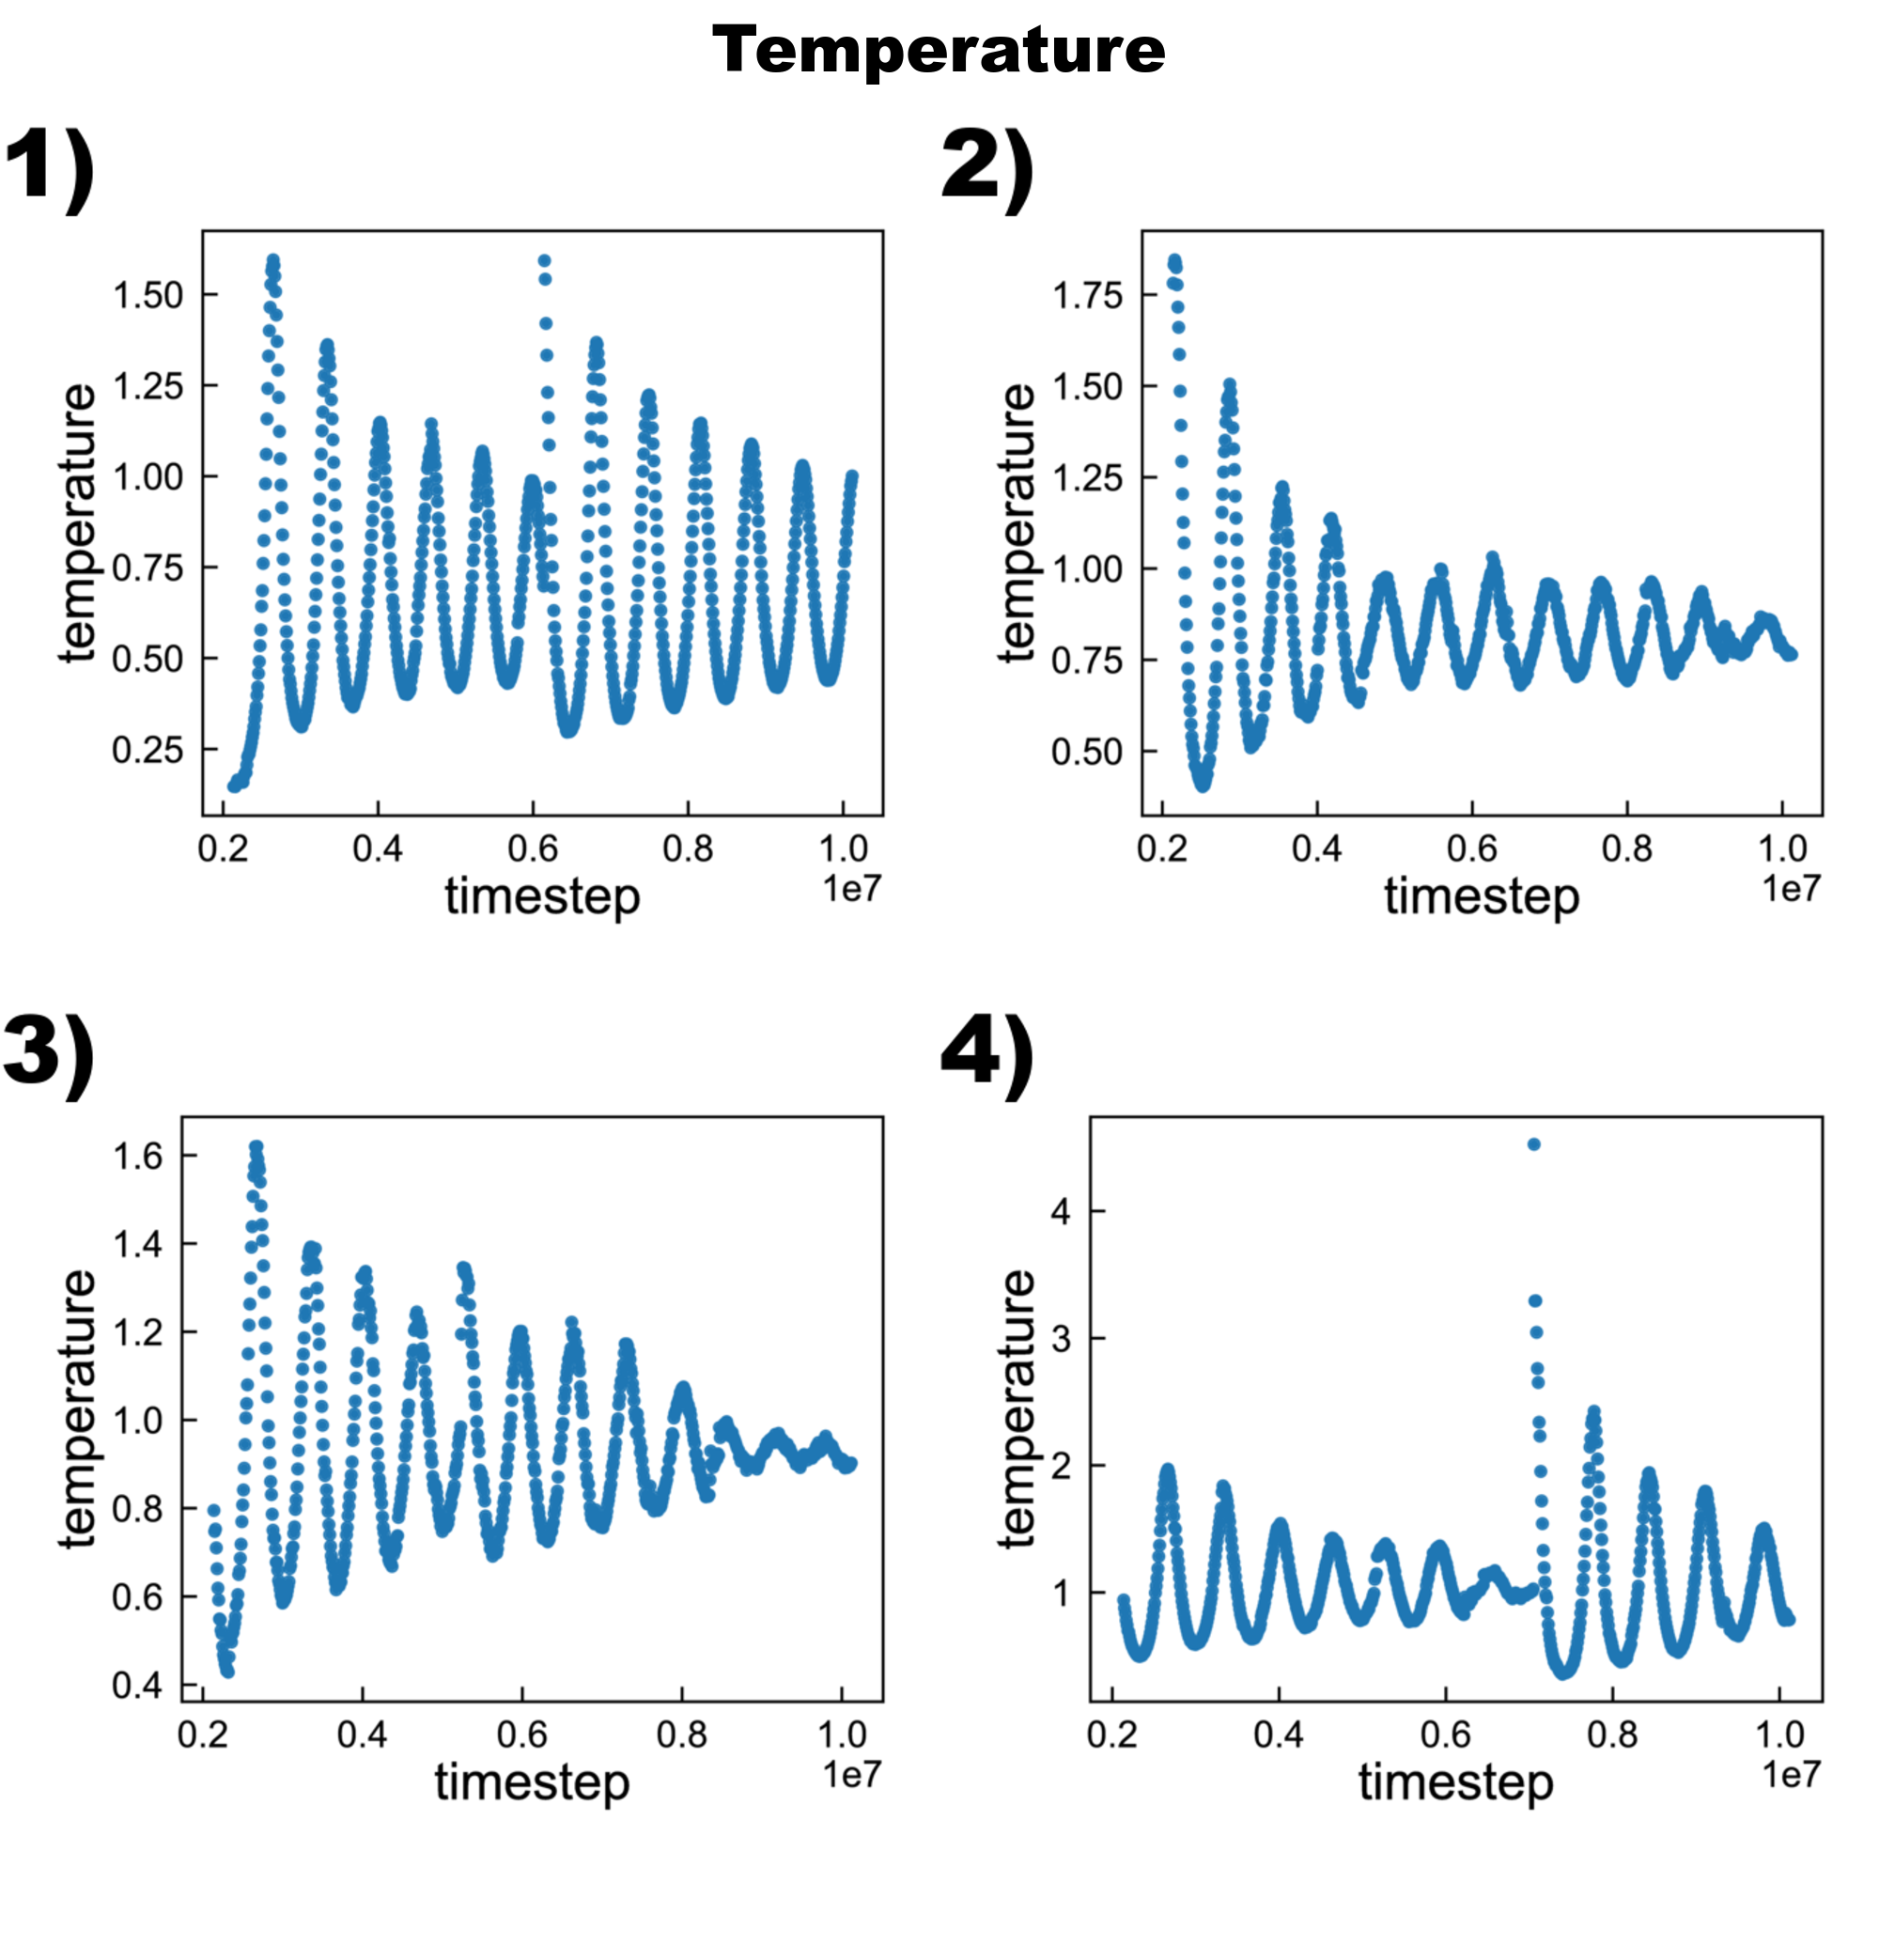
\includegraphics[width=\textwidth]{Figures/Temperature.png}
    \caption{The evolution of the temperature of the p1-L15-f0.0-P0.1-TX.X-e0.5 systems.
        a) $T = 1.5$, b) $T = 1.75$, c) $T = 2.0$, d) $T = 2.25$.
    The temperature was dumped 1000 times for each phase, and only the final 800 energy values recorded are shown here.
    The final phase ran 1E7 timesteps of 1E-5s each.
}
	\label{fig:T}
\end{figure}


\begin{figure}[h!]\centering
	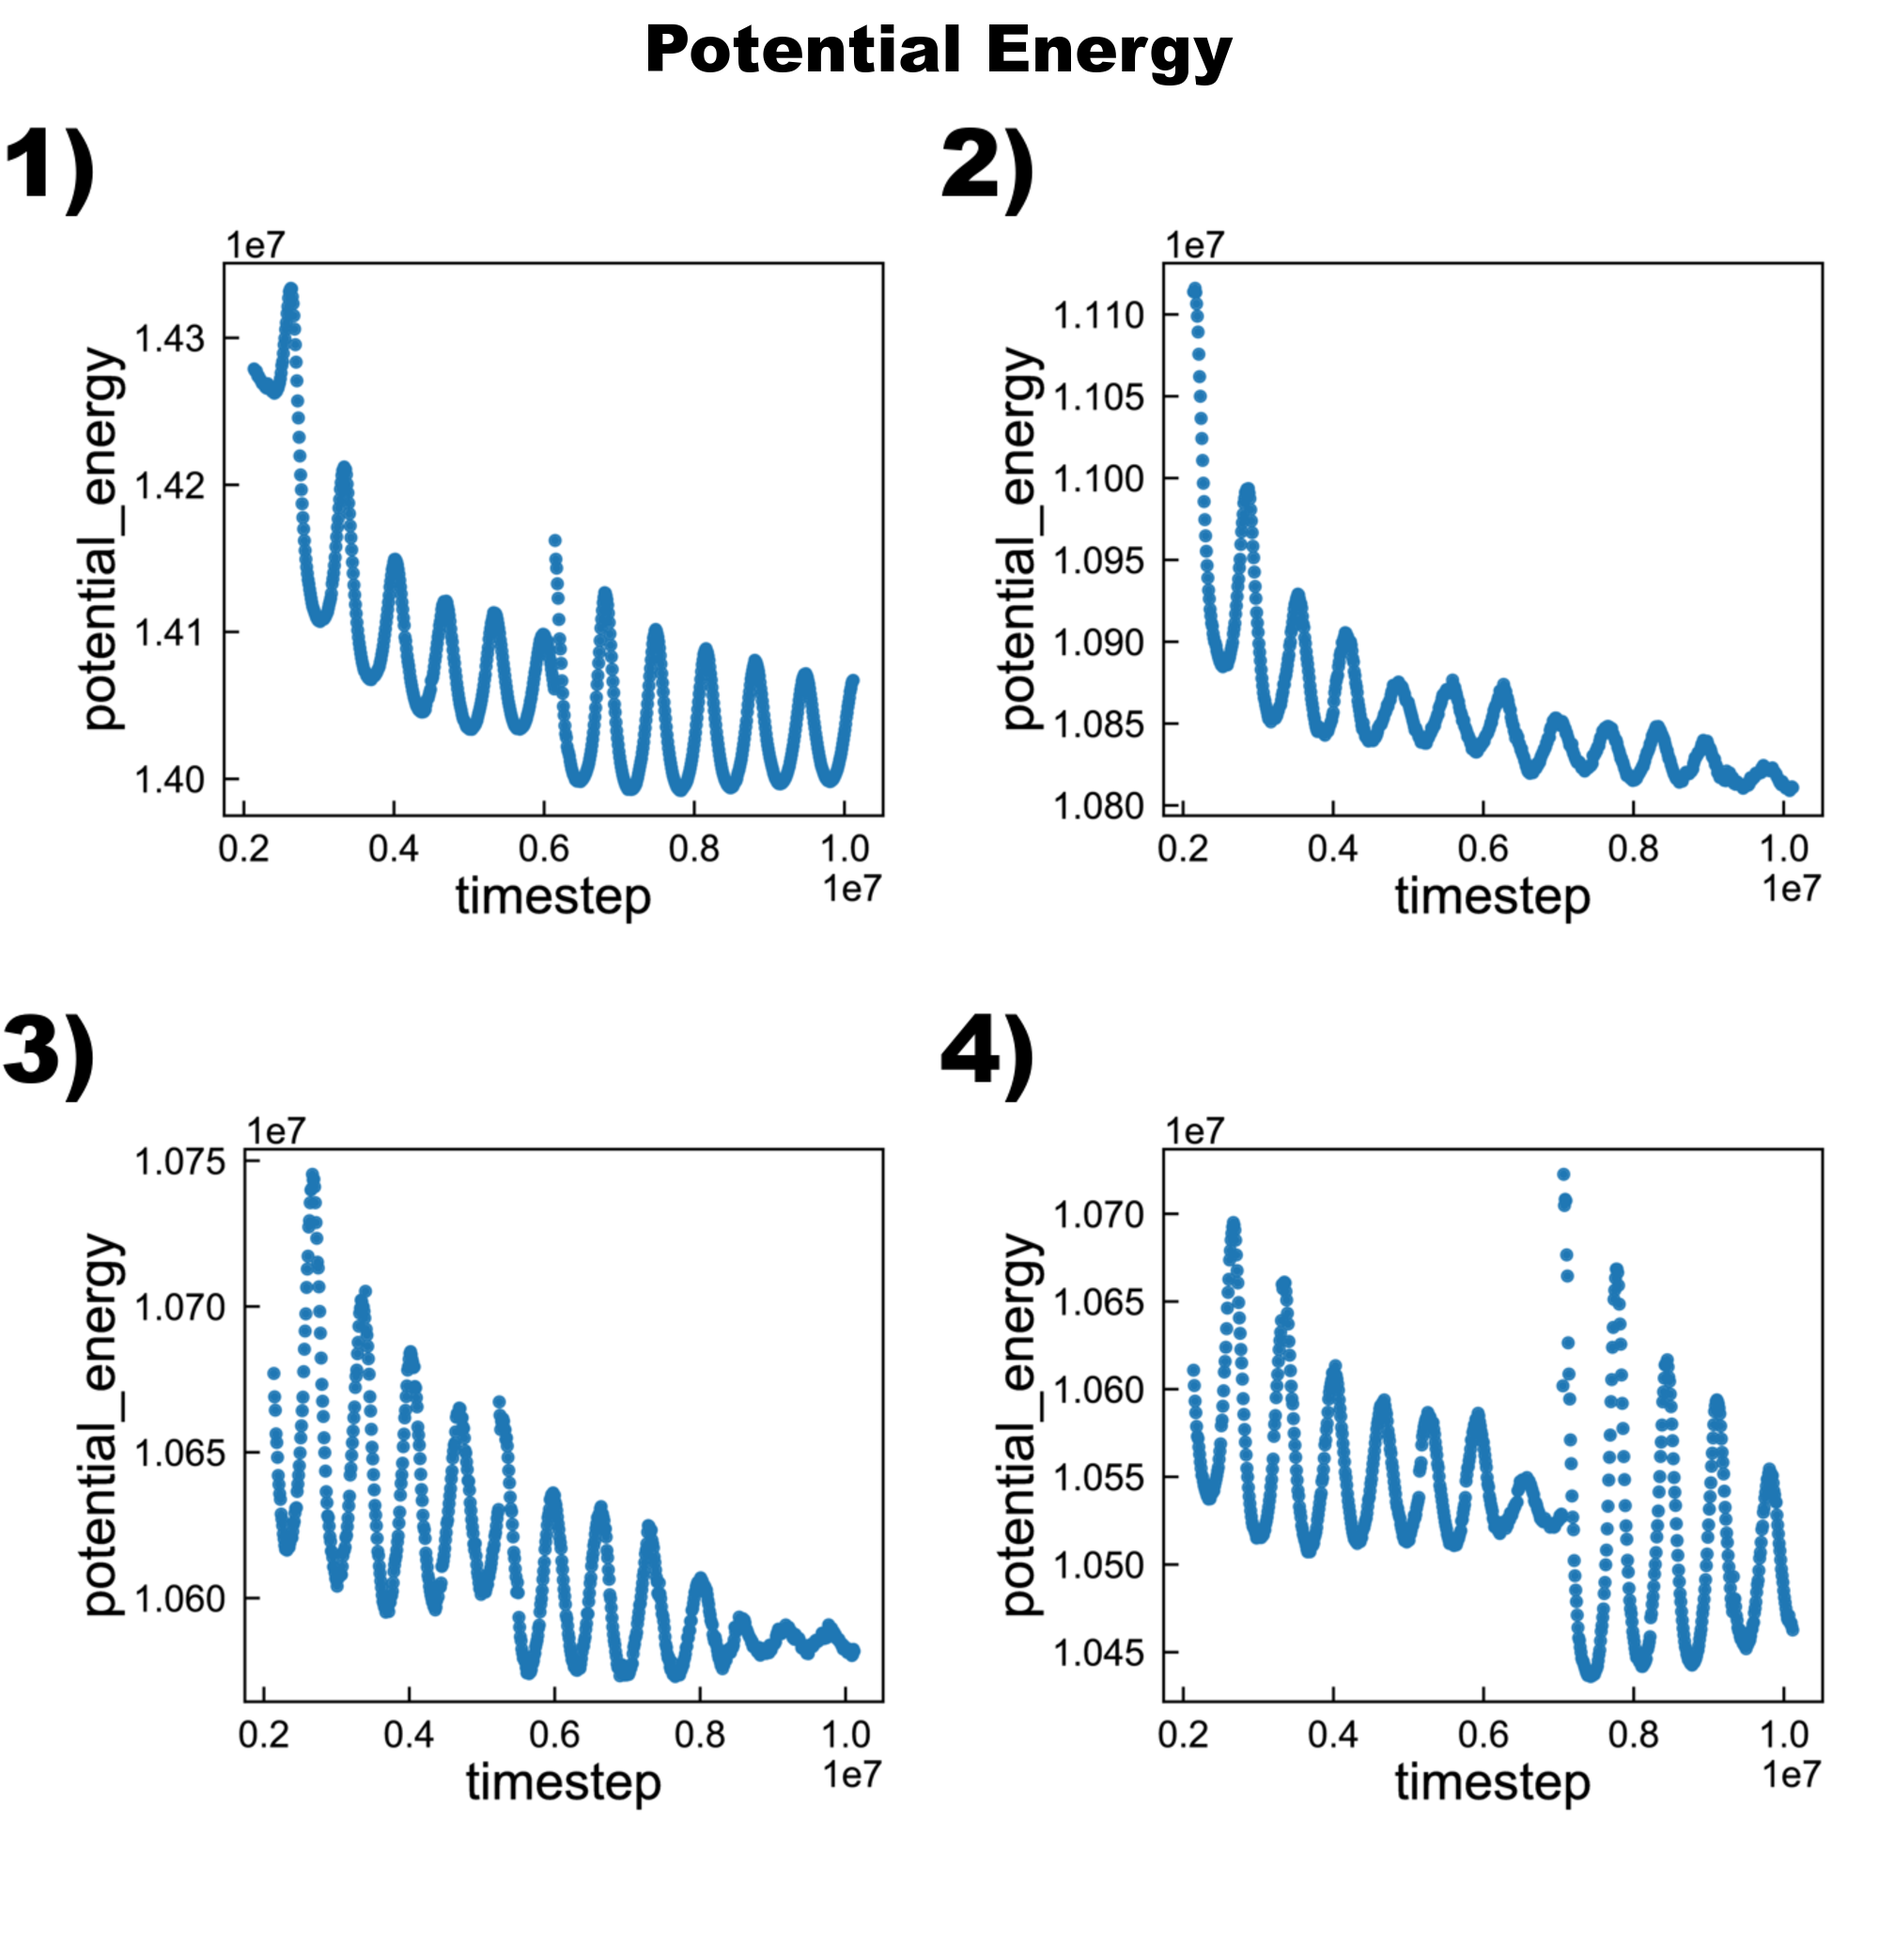
\includegraphics[width=\textwidth]{Figures/Potential_Energy.png}
    \caption{The evolution of the total potential energy of the p1-L15-f0.0-P0.1-TX.X-e0.5 systems.
        a) $T = 1.5$, b) $T = 1.75$, c) $T = 2.0$, d) $T = 2.25$.
    The potential energy was dumped 1000 times for each phase, and only the final 800 energy values recorded are shown here.
    The final phase ran 1E7 timesteps of 1E-5s each.
}
	\label{fig:PE}
\end{figure}


\textcolor{red}{Not going to report the mobilities until we are happy with the equilibration first.}


\bibliography{refs}
\bibliographystyle{unsrt}


\end{document}
